
% Lab 1 Handout

\labtitle{\semester}{1}{Monday, August 31/Tuesday, September 1}

\section*{Learning Goals}
During this lab, you will:
\begin{itemize}
    \item approach problems with consideration for runtime complexity
    \item apply sorting as a tool for solving some real problems
    \item consider tradeoffs between different solutions to problems
    \item get a feel for the sort of problem solving that this course will focus on
\end{itemize}

\section*{Problem 0: General Approaches}

When faced with these sorts of algorithmic problems, there are some general considerations to take:
\begin{itemize}
    \item Is there a known algorithm that solves this problem, or a related problem?
    \item Which kinds of data structures fit the operations we need to do?
    \item Do we have bounds on our input or on our runtime requirement?
    \item Does the problem give us additional information that might help us do better?
    \item Ignoring efficiency considerations, what is the very first working solution you can come up with?
\end{itemize}

\section*{Problem 1: Unique Character Strings}
\textit{Given a string of length $n$, determine whether it contains all unique characters – or, whether any characters are used more than once.}\\\\
\uline{Food for Thought:}
\begin{itemize}
    \item If you do it as fast as possible, how much extra space is needed?
    \item If you do it with no extra space, how quickly can you do it?
    \item What if you aren't worried about destroying the input string?
\end{itemize}

\section*{Problem 2: Anagram Strings}
\textit{Given two strings, determine whether they are anagrams of each other.}

\begin{center}
    \uline{Example:}\\

    \texttt{TOMMARVOLORIDDLE} $\longleftrightarrow$ \texttt{IAMLORDVOLDEMORT}\\

    \textit{The above are anagrams of each other!\\ (Sorry if we spoiled book 2 of Harry Potter for you...)}
\end{center}

\begin{itemize}
    \item If you do it as fast possible, how much extra space is needed?
    \item If you do it with no extra space, how quickly can you do it?
    \item What if you aren't worried about destroying the input strings?
\end{itemize}

\section*{Problem 3: Dutch National Flag Problem}
\textit{Given $n$ balls of three colors – say red, white, and blue – arranged randomly in a line, sort them as quickly as possible into contiguous groups of red, white, and blue, with the groups in that order.}

\begin{figure}[h]
    \centering
    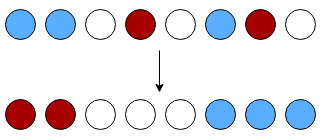
\includegraphics[width=\textwidth*3/8]{dutch_flag}
\end{figure}

\begin{itemize}
    \item How fast can generic sorts do this?
    \item What additional information do we have, beyond what generic sorts assume?
    \item Can we sort it in-place in $O(n)$ time?
\end{itemize}

\section*{Problem 4: Row/Column-sorted Matrix Membership}
\textit{Given an $m$ by $n$ matrix of integers, where each row and each column of the matrix is sorted, determine whether an integer $k$ exists somewhere in the matrix.}
\begin{itemize}
    \item How could we do this if we didn't know the rows and columns were sorted?
    \item How does knowing the rows and columns are sorted let us do this faster?
    \item What is our optimal runtime?
\end{itemize}
    
